% !Mode:: "TeX:UTF-8"
% 请注意,此文件的编码方式一定要设置为UTF-8 无DOM模式
% 否则中文显示乱码!
% 可以用notepad++ 或ultraedit查看/更改文件编码方式

\documentclass[a4paper,12pt]{article}

%插入超链接,并且去除超链接的颜色下划线等特性
\usepackage[hidelinks]{hyperref}

%该宏包可以添加伪代码CLRS《算法导论》**第三版**模式
%clrscode3e.sty放在项目根目录下即可
\usepackage{clrscode3e}

%插入数学公式
\usepackage{amsmath}

%中文包
\usepackage{xeCJK}
\setCJKmainfont{SimSun}

%设置页边距
\usepackage[top=0.7in,bottom=0.8in,left=1.1in,right=1in]{geometry}

\usepackage{xcolor}

%为了插入代码
\usepackage{listings}

\definecolor{codegreen}{rgb}{0,0.6,0}
\definecolor{codegray}{rgb}{0.5,0.5,0.5}
\definecolor{codepurple}{rgb}{0.58,0,0.82}
\definecolor{backcolour}{rgb}{0.95,0.95,0.92}

\lstdefinestyle{mystyle}{
    backgroundcolor=\color{backcolour},
    commentstyle=\itshape\color{codegreen},
    keywordstyle=\color{magenta},
    numberstyle=\tiny\color{codegray},
    stringstyle=\color{codepurple},
    basicstyle=\footnotesize,
    breakatwhitespace=false,
    breaklines=true,
    captionpos=b,
    keepspaces=true,
    numbers=left,
    numbersep=5pt,
    showspaces=false,
    showstringspaces=false,
    showtabs=false,
    tabsize=4
}

\lstdefinestyle{default}{
    backgroundcolor=\color{backcolour},
    commentstyle=\itshape,
    numberstyle=\tiny,
    basicstyle=\footnotesize,
    breakatwhitespace=false,
    breaklines=true,
    captionpos=b,
    keepspaces=true,
    numbers=left,
    numbersep=5pt,
    showspaces=false,
    showstringspaces=false,
    showtabs=false,
    tabsize=4
}

\lstset{style=mystyle}

%为了插入图片
%\usepackage{graphicx}

%首段缩进
\usepackage{indentfirst}

%为了画图
\usepackage{tikz}
\usetikzlibrary{positioning}

\title{Assignment 5\\Algorithm Design and Analysis}

\author{\href{http://bitjoy.net}{bitjoy.net}}
\date{December 16, 2015}

\begin{document}

\maketitle

I choose problem 1,2,5,7,8,9.

\section*{1\quad Problem Reduction}
\subsection*{\textnormal{1.1\quad Algorithm description}}

We first construct a bipartite graph by linking the girl and the boys who the girl likes. For example, girl 1 likes boy 5 and boy 6, then edge(1,5) and edge(1,6) are added. After that, add node $s$ and $t$ and connect $s$ with girls and $t$ with boys. Set each edge's capacity as 1, then we get a extended network. Figure 1 shows an example.

%http://tex.stackexchange.com/questions/8652/what-does-t-and-ht-mean
\begin{figure}[!ht]
\centering
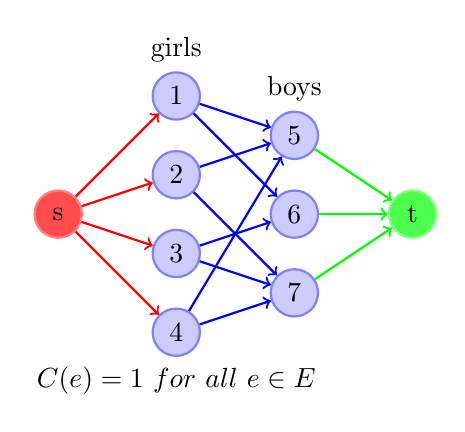
\begin{tikzpicture}
    [girl/.style={circle, draw=blue!50,fill=blue!20,thick,inner sep=0pt,minimum size=6mm},
    boy/.style={circle, draw=blue!50,fill=blue!20,thick,inner sep=0pt,minimum size=6mm},
    s/.style={circle, draw=red!50,fill=red!70,thick,inner sep=0pt,minimum size=6mm},
    t/.style={circle, draw=green!50,fill=green!70,thick,inner sep=0pt,minimum size=6mm}]
    \node[s] (s) at (-0.5,0) {s};
    \node[girl] (g2) at (1,0.5) {2};
    \node[girl, label=girls] (g1) at (1,1.5) {1};
    \node[girl] (g3) at (1,-0.5) {3};
    \node[girl, label=below:{$C(e)=1~for~all~e \in E$}] (g4) at (1,-1.5) {4};
    \node[boy] (b6) at (2.5,0) {6};
    \node[boy, label=boys] (b5) at (2.5,1) {5};
    \node[boy] (b7) at (2.5,-1) {7};
    \node[t] (t) at (4,0) {t};

    \draw [->,red,thick] (s) -- (g1);
    \draw [->,red,thick] (s) -- (g2);
    \draw [->,red,thick] (s) -- (g3);
    \draw [->,red,thick] (s) -- (g4);

    \draw [->,blue,thick] (g1) -- (b5);
    \draw [->,blue,thick] (g1) -- (b6);
    \draw [->,blue,thick] (g2) -- (b5);
    \draw [->,blue,thick] (g2) -- (b7);
    \draw [->,blue,thick] (g3) -- (b6);
    \draw [->,blue,thick] (g3) -- (b7);
    \draw [->,blue,thick] (g4) -- (b5);
    \draw [->,blue,thick] (g4) -- (b7);

    \draw [->,green,thick] (b5) -- (t);
    \draw [->,green,thick] (b6) -- (t);
    \draw [->,green,thick] (b7) -- (t);
\end{tikzpicture}
\caption{Extended network for maximal matching.}
\end{figure}

As a result, the maximum flow of the extended network is the maximum matching, we can run Ford-Fulkerson Algorithm to find the answer.

To summarize, we have the following algorithm, $G$ is the original bipartite graph.
\begin{codebox}
\Procname{$\proc{MAX-MATCHING}(G)$}
\li adding node $s$ and $t$ to $G$
\li connecting $s$ with girls and $t$ with boys
\li setting the capacity of edges equals to 1 for all edges in $G$
\li running Ford-Fulkerson Algorithm to find the maximum flow in $G$
\li \Return the maximum flow as the maximum matching
\end{codebox}

\subsection*{\textnormal{1.2\quad Correctness of the algorithm}}

By setting the capacity of each edge as 1, we can assure that each girl appears at most in one pair, so does each boy. So, the maximum flow of the extended network equals to the number of edges between girls and boys, which is the maximum matching between them.

\subsection*{\textnormal{1.3\quad Complexity of the algorithm}}

As we know, the time complexity of Ford-Fulkerson Algorithm is $O(E|f^*|)$ where $E$ is the number of edges in $G$ and $|f^*|$ is the maximum flow.

In algorithm MAX-MATCHING, we just add two nodes, say $s$ and $t$, and connect some nodes to $s$, others to $t$, it takes $O(V)$ where $V$ is the number of nodes in $G$. So, the total time complexity is $O(E|f^*|+V)$.

\section*{2\quad Problem Reduction}
\subsection*{\textnormal{2.1\quad Algorithm description}}


Similar to Problem 1, we construct a extended network like Figure 2:

%http://tex.stackexchange.com/questions/8652/what-does-t-and-ht-mean
\begin{figure}[!ht]
\centering
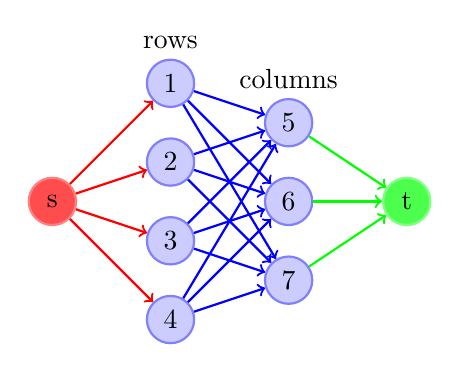
\begin{tikzpicture}
    [row/.style={circle, draw=blue!50,fill=blue!20,thick,inner sep=0pt,minimum size=6mm},
    column/.style={circle, draw=blue!50,fill=blue!20,thick,inner sep=0pt,minimum size=6mm},
    s/.style={circle, draw=red!50,fill=red!70,thick,inner sep=0pt,minimum size=6mm},
    t/.style={circle, draw=green!50,fill=green!70,thick,inner sep=0pt,minimum size=6mm}]
    \node[s] (s) at (-0.5,0) {s};
    \node[row] (r2) at (1,0.5) {2};
    \node[row, label=rows] (r1) at (1,1.5) {1};
    \node[row] (r3) at (1,-0.5) {3};
    \node[row] (r4) at (1,-1.5) {4};
    \node[column] (c6) at (2.5,0) {6};
    \node[column, label=columns] (c5) at (2.5,1) {5};
    \node[column] (c7) at (2.5,-1) {7};
    \node[t] (t) at (4,0) {t};

    \draw [->,red,thick] (s) -- (r1);
    \draw [->,red,thick] (s) -- (r2);
    \draw [->,red,thick] (s) -- (r3);
    \draw [->,red,thick] (s) -- (r4);

    \draw [->,blue,thick] (r1) -- (c5);
    \draw [->,blue,thick] (r1) -- (c6);
    \draw [->,blue,thick] (r1) -- (c7);
    \draw [->,blue,thick] (r2) -- (c5);
    \draw [->,blue,thick] (r2) -- (c6);
    \draw [->,blue,thick] (r2) -- (c7);
    \draw [->,blue,thick] (r3) -- (c5);
    \draw [->,blue,thick] (r3) -- (c6);
    \draw [->,blue,thick] (r3) -- (c7);
    \draw [->,blue,thick] (r4) -- (c5);
    \draw [->,blue,thick] (r4) -- (c6);
    \draw [->,blue,thick] (r4) -- (c7);

    \draw [->,green,thick] (c5) -- (t);
    \draw [->,green,thick] (c6) -- (t);
    \draw [->,green,thick] (c7) -- (t);
\end{tikzpicture}
\caption{Extended network for matrix construction. $C(e) = 1$ for all edges between rows and columns, $C(<s,r>) = row\_sum[r]$, $C(<c,t>) = column\_sum[c]$.}
\end{figure}

As matrix can only be filled with 0 or 1, the capacity of edges between rows and columns equals to 1, the capacity out from $s$ equals to each row sum and the capacity into $t$ equals to each column sum. Given the 4*3 matrix, we have Figure 2.

We can get the maximum flow by running Ford-Fulkerson algorithm, if the maximum flow equals to the sum of all row sums(or all column sums), the final flow graph is the matrix we want.

To summarize, we have the following algorithm, R and C for the number of rows and columns, R\_SUM and C\_SUM for the list of sum of rows and columns.

\begin{codebox}
\Procname{$\proc{MATRIX-CONSTRUCTION}(R,C,R\_SUM,C\_SUM)$}
\li constructing a graph $G$ with $R+C+2$ nodes, node 0 for $s$, node $R+C+1$ for $t$,
\zi ~~~~node $1\sim R$ for rows and node $R+1\sim R+C$ for columns
\li connecting $s$ with rows, $t$ with columns and all rows with all columns
\li setting $C(e) = 1$ for all edges between rows and columns,
\zi ~~~~$C(<s,r>) = R\_SUM[r]$, $C(<c,t>) = C\_SUM[c]$
\li running Ford-Fulkerson Algorithm to find the maximum flow in $G$
\li \If max-flow == sum of R\_SUM
    \Then
\li \Return the final flow graph
\li \Else
    \Return No matrix found!
    \End
\end{codebox}

\subsection*{\textnormal{2.2\quad Correctness of the algorithm}}

By setting the capacity of edges between rows and columns as 1, we can assure that only 0 or 1 will be filled in the matrix. So, the maximum flow of the extended network equals to the sum of all elements in the matrix. If the max flow equals to the sum of all row sums required, then the matrix is found, otherwise, no matrix meets the requirements.

\subsection*{\textnormal{2.3\quad Complexity of the algorithm}}

Similar to problem 1, the time complexity of MATRIX-CONSTRUCTION algorithm is $O(E|f^*|+V)$.

\section*{5\quad Dogs and kennels}
\subsection*{\textnormal{5.1\quad Algorithm description}}

Suppose one dog stands at $(x_1,y_1)$ and one kennel is placed at $(x_2,y_2)$, then their distance is $(|x_1-x_2|,|y_1-y_2|)$. As 1 fee per step, once we get all distance between $n$ dogs and $n$ kennels, we get the cost between them.

So the problem is transferred to minimum cost flow. We construct a extended network like Figure 3:

%http://tex.stackexchange.com/questions/8652/what-does-t-and-ht-mean
\begin{figure}[!ht]
\centering
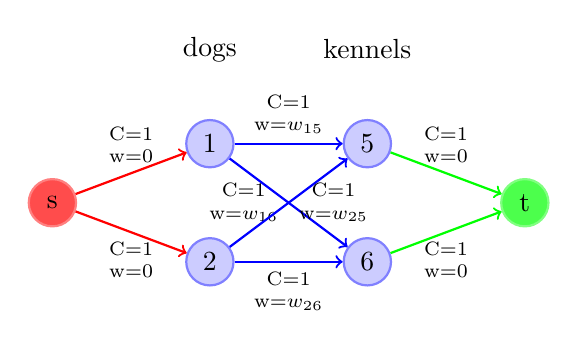
\begin{tikzpicture}
    [dog/.style={circle, draw=blue!50,fill=blue!20,thick,inner sep=0pt,minimum size=6mm},
    kennel/.style={circle, draw=blue!50,fill=blue!20,thick,inner sep=0pt,minimum size=6mm},
    s/.style={circle, draw=red!50,fill=red!70,thick,inner sep=0pt,minimum size=6mm},
    t/.style={circle, draw=green!50,fill=green!70,thick,inner sep=0pt,minimum size=6mm},
    txt/.style={}]
    \node[s] (s) at (-1,1.25) {s};
    \node[dog] (d2) at (1,0.5) {2};
    \node[dog] (d1) at (1,2) {1};
    \node[kennel] (k6) at (3,0.5) {6};
    \node[kennel] (k5) at (3,2) {5};
    \node[t] (t) at (5,1.25) {t};
    \node[txt] (dogs) at (1,3.2) {dogs};
    \node[txt] (kennels) at (3,3.2) {kennels};

    \draw [->,red,thick] (s) -- (d1) node[above,font=\scriptsize,color=black,align=center,midway]{C=1\\w=0};
    \draw [->,red,thick] (s) -- (d2) node[below,font=\scriptsize,color=black,align=center,midway]{C=1\\w=0};

    \draw [->,blue,thick] (d1) -- (k5) node[above,font=\scriptsize,color=black,align=center,midway]{C=1\\w=$w_{15}$};
    \draw [->,blue,thick] (d1) -- (k6) node[left,font=\scriptsize,color=black,align=center,midway]{C=1\\w=$w_{16}$};
    \draw [->,blue,thick] (d2) -- (k5) node[right,font=\scriptsize,color=black,align=center,midway]{C=1\\w=$w_{25}$};
    \draw [->,blue,thick] (d2) -- (k6) node[below,font=\scriptsize,color=black,align=center,midway]{C=1\\w=$w_{26}$};

    \draw [->,green,thick] (k5) -- (t) node[above,font=\scriptsize,color=black,align=center,midway]{C=1\\w=0};
    \draw [->,green,thick] (k6) -- (t) node[below,font=\scriptsize,color=black,align=center,midway]{C=1\\w=0};
\end{tikzpicture}
\caption{Extended network for dogs and kennels. $C(e) = 1$ for all edges, cost between dogs and kennels equals to their distance.}
\end{figure}

Set capacity as 1 for all edges, so that one dog can only enter one kennel and one kennel can only accommodate one dog. The objective of the network is to transfer $v_0=n$ dogs to $n$ kennels from $s$ to $t$ with minimal cost, which we can run minimum cost flow algorithm such as Klein's \emph{Cycle canceling} algorithm to obtain it.

To summarize, we have the following algorithm, $D$ and $K$ are dogs' and kennels' position respectively, $s$ and $t$ are source and sink respectively.

\begin{codebox}
\Procname{$\proc{SEND-DOGS-TO-KENNELS}(D, K, s, t)$}
\li \For $d \in D$
    \Then
\li (s,d).C = 1
\li (s,d).w = 0
    \End
\li \For $k \in K$
    \Then
\li (k,t).C = 1
\li (k,t).w = 0
    \End
\li \For $d \in D$
    \Then
\li \For $k \in K$
    \Then
\li (d,k).C = 1
\li (d,k).w = dist(d,k)
    \End
    \End
\li running minimum cost flow algorithm
\zi ~~~~to find a circulation $f$ with flow value $v_0=n$ and the cost is minimized
\li \Return the minimum cost
\end{codebox}

\subsection*{\textnormal{5.2\quad Correctness of the algorithm}}

By setting the capacity of all edges as 1, we can assure that one dog only enters one kennel and one kennel only accommodates one dog. By setting the objective flow as $v_0=n$, we can assure all $n$ dogs find their kennels. Once minimize the cost, we get the minimum money to send these $n$ little dogs into those $n$ different kennels.

Note since $s$ and $t$ are virtual nodes, their edges' weights equal to 0.

\subsection*{\textnormal{5.3\quad Complexity of the algorithm}}

As we know, the complexity of \emph{Cycle canceling} algorithm is $O(E^2VCW)$ where $E,V$ are the number of edges and vertexes respectively, $C,W$ are the maximal capacity and cost respectively.

In SEND-DOGS-TO-KENNELS algorithm, $E=n^2+2n$, $V=2n+2$ and $C=1$, so \emph{Cycle canceling} costs $O(Wn^5)$. What's more, we have four extra $for$ loops, which cost $O(n^2)$, so the total time complexity is $O(Wn^5+n^2)=O(Wn^5)$ where $W$ is the maximal distance between dogs and kennels.

\section*{7\quad Maximum flow}

The dual of primal problem is:

\[
\begin{array}{rrrrrrrrl}
\min & y & = &\sum u_ed_e & &\\
s.t. & \sum\limits_{e\in P}d_e & \geq & 1 & (\forall P)\\
& d_e & \geq& 0 & (\forall e)
\end{array}
\]

where $y$ is the value that we optimize, $u_e$ is the capacity of edge $e$ and $d_e$'s are variables.

This is LP formulation for minimum $s-t$ cut. Let the cut-set be $C=\{(u,v)\in E | u\in S, v\in T\}$, if $e\in C$ then $d_e=1$, otherwise 0.

The first constraint says that there must be at least one edge in cut-set $C$ from one path $P$, which is obvious. The second constraint says that each edge is nonnegative.

By strong duality, the minimum capacity over all $s-t$ cuts is equal to the maximum value of an $s-t$ flow\footnote{\href{https://en.wikipedia.org/wiki/Max-flow_min-cut_theorem}{https://en.wikipedia.org/wiki/Max-flow\_min-cut\_theorem}}.

\section*{8\quad Ford-Fulkerson algorithm}

I implemented the Ford-Fulkerson algorithm in Python 3.

\begin{lstlisting}[language=python]
# -*- coding: utf-8 -*-
"""
Created on Mon Dec 14 21:21:27 2015

@author: czl
"""

# use numpy to handle data structure
import numpy as np
from collections import deque

# BFS finds a path and its bottleneck
def BFS(G, s, t):
    dq = deque([[[s], np.inf]])
    while len(dq) > 0:
        path, cf = dq.popleft()
        tmp = path[-1]
        if tmp == t:
            return True, path, cf
        else:
            for j in range(G.shape[1]):
                if j not in path and G[tmp][j] > 0:
                    dq.append([path + [j], min(cf, G[tmp][j])])
    return False, [], np.inf

# find max flow in directed graph G
def Ford_Fulkerson(G, s, t):
    flag, path, cf = BFS(G, s, t) # G is residual network Gf
    while flag:
        #print(G)
        #print(path)
        for i in range(len(path) - 1):
            u = path[i]
            v = path[i + 1]
            G[u][v] -= cf
            G[v][u] += cf
        flag, path, cf = BFS(G, s, t)
    max_flow = 0
    for j in range(G.shape[1]):
        max_flow += G[j][s]
    return max_flow

if __name__ == "__main__":
    f = open('./problem1.data')
    for i in range(3):
        f.readline()
    while True:
        line = f.readline()
        if not line:
            break
        girls, boys = line.split(' ')
        girls = int(girls)
        boys = int(boys)
        G = np.zeros([girls + boys + 2] * 2, dtype=np.int)
        s = 0
        t = girls + boys + 1
        for girl in range(girls):
            G[s][girl + 1] = 1
            line = f.readline().rstrip('\n')
            b = line.split(' ')
            b = list(map(int, b))
            for boy in range(b[0]):
                G[girl + 1][girls + b[boy + 1]] = 1
        for boy in range(boys):
            G[girls + boy + 1][t] = 1
        print(Ford_Fulkerson(G, s, t))
    f.close()
\end{lstlisting}

If you want to list the intermediate steps, just uncomment line 30 and line 31.The answers to problem 1 gotten by my implementation show below:
\\
2\\
9\\
11\\
16\\
18\\
116

\section*{9\quad Push-relabel}

I implemented the Push-relabel algorithm in Python 3.

\begin{lstlisting}[language=python]
# -*- coding: utf-8 -*-
"""
Created on Tue Dec 15 14:51:33 2015

@author: czl
"""

# use numpy to handle data structure
import numpy as np

def push(Gf, height, excess_flow, u):
    if excess_flow[u] <= 0:
        return False
    for v in range(len(Gf)):
        if v != u and Gf[u][v] > 0 and height[u] == height[v] + 1:
            df = min(excess_flow[u], Gf[u][v])
            Gf[u][v] -= df
            Gf[v][u] += df
            excess_flow[u] -= df
            excess_flow[v] += df
            return True
    return False

def relabel(Gf, height, excess_flow, u):
    if excess_flow[u] <= 0:
        return False
    min_h = np.inf
    for v in range(len(Gf)):
        if v != u and Gf[u][v] > 0:
            if height[u] > height[v]:
                return False
            else:
                min_h = min(min_h, height[v])
    height[u] = min_h + 1
    return True


def initialize_preflow(G, s):
    n = len(G)
    height = [0] * n
    excess_flow = [0] * n
    height[s] = n
    for v in range(n):
        if v != s and G[s][v] != 0:
            excess_flow[v] = G[s][v]
            excess_flow[s] -= G[s][v]
            G[v][s] = G[s][v]
            G[s][v] = 0
    return G, height, excess_flow


def generic_push_relabel(G, s, t):
    G_original = np.copy(G)
    n = len(G)
    Gf, height, excess_flow = initialize_preflow(G, s)
    while True:
        push_or_relabel = False
        for u in range(n):
            if u != s and u != t:
                if push(Gf, height, excess_flow, u):
                    push_or_relabel = True
                    break
                if relabel(Gf, height, excess_flow, u):
                    push_or_relabel = True
                    break
        if not push_or_relabel:
            break
#        else:
#            print(Gf)
    max_flow = 0
    for j in range(n):
        max_flow += Gf[j][s]
    G_flow = np.zeros(G.shape, dtype=np.int)
    for row in range(G.shape[0]):
        for col in range(G.shape[1]):
            if G_original[row][col] != 0:
                G_flow[row][col] = G_original[row][col] - Gf[row][col]
    return max_flow, G_flow


if __name__ == "__main__":
    f = open('./problem2.data')
    ans = open('./problem2.answer', 'ab')
    for i in range(3):
        f.readline()
    while True:
        line = f.readline()
        if not line:
            break
        R, C = line.split(' ')
        R = int(R)
        C = int(C)
        G = np.zeros([R + C + 2] * 2, dtype=np.int)
        line = f.readline().rstrip(' \n')
        R_SUM = list(map(int, line.split(' ')))
        line = f.readline().rstrip(' \n')
        C_SUM = list(map(int, line.split(' ')))
        s = 0
        t = R + C + 1
        for row in range(R):
            G[s][row + 1] = R_SUM[row]
        for col in range(C):
            G[R + col + 1][t] = C_SUM[col]
        for row in range(1, R + 1):
            for col in range(R + 1, R + C + 1):
                G[row][col] = 1
        max_flow, G_flow = generic_push_relabel(G, s, t)
        matrix = G_flow[1 : R + 1, R + 1 : R + C + 1]
        #print(matrix)
        np.savetxt(ans, matrix, delimiter=',', fmt='%d')
        ans.write(bytes('-----------------------------------\n', 'UTF-8'))
        if max_flow == sum(R_SUM):
            print('Answer is right!')
        else:
            print('Answer is wrong!')
    f.close()
    ans.close()
\end{lstlisting}

If you want to list the intermediate steps, just uncomment line 68 and line 69.The first answer to problem 2 gotten by my implementation shows below:
\[
\begin{bmatrix}
1&0&0&0&0&0&1&1&1&1\\
1&0&0&0&0&0&1&1&1&1\\
1&0&0&0&1&1&1&1&1&1\\
1&0&1&0&0&1&1&1&1&1\\
0&1&1&1&1&1&0&0&0&1\\
0&1&1&0&0&1&0&0&0&0\\
0&1&1&1&1&0&0&0&0&1\\
0&1&1&1&1&1&1&0&0&1\\
1&1&1&1&1&1&1&0&0&0\\
1&1&1&0&0&0&0&0&0&0
\end{bmatrix}
\]

For more details, please see file \href{run:./problem2.answer}{$problem2.answer$}. According to the pseudo code of problem 2, if the maximum flow of the extended network equals to the sum of all row sums, the answer is right. I have checked my answers, all of them are right.
\end{document}
